% ============================================================================
%  Dissertation defence slides
%  Build with:  latexmk -xelatex slides.tex      (XeLaTeX, for the diacritics)
%
%  Target: 10-12 minutes.  See TIMING notes marked [OPTIONAL] -- those frames
%  can be dropped or shown without comment if you are running long.
% ============================================================================
\documentclass[aspectratio=169, 11pt]{beamer}

\usepackage{fontspec}
\usepackage{amsmath, amssymb}
\usepackage{booktabs}
\usepackage{multirow}
\usepackage{tikz}
\usetikzlibrary{arrows.meta, positioning, shapes.geometric}
\usepackage{appendixnumberbeamer}

% ---------------------------------------------------------------- theme ----
\usetheme{default}
\usecolortheme{default}
\setbeamertemplate{navigation symbols}{}
\setbeamertemplate{itemize items}[circle]
\setbeamertemplate{itemize subitem}[triangle]

\definecolor{accent}{HTML}{1F4E79}
\definecolor{accentlight}{HTML}{4C8FD1}
\definecolor{warm}{HTML}{E07B39}
\definecolor{ink}{HTML}{262626}

\setbeamercolor{structure}{fg=accent}
\setbeamercolor{frametitle}{fg=accent, bg=white}
\setbeamercolor{title}{fg=accent}
\setbeamercolor{normal text}{fg=ink}
\setbeamercolor{alerted text}{fg=warm}
\setbeamerfont{frametitle}{size=\large, series=\bfseries}
\setbeamerfont{framesubtitle}{size=\small, shape=\itshape}
\setbeamercolor{framesubtitle}{fg=gray}

% blocks need a visible ground: the default theme draws them as bare text
\setbeamertemplate{blocks}[rounded][shadow=false]
\setbeamercolor{block title}{fg=white, bg=accent}
\setbeamercolor{block body}{fg=ink, bg=accent!7}

% a thin rule under each frame title
\makeatletter
\setbeamertemplate{frametitle}{%
  \vspace{0.6em}%
  \begin{minipage}{\textwidth}%
    \usebeamerfont{frametitle}\usebeamercolor[fg]{frametitle}\insertframetitle\par
    \ifx\insertframesubtitle\@empty\else
      \vspace{0.12em}%
      \usebeamerfont{framesubtitle}\usebeamercolor[fg]{framesubtitle}%
      \insertframesubtitle\par
    \fi
    \vspace{0.25em}%
    {\color{accent!35}\rule{\textwidth}{0.6pt}}%
  \end{minipage}%
}
\makeatother

% page number, bottom right
\setbeamertemplate{footline}{%
  \hfill{\color{gray}\scriptsize\insertframenumber/\inserttotalframenumber}%
  \hspace{1.2em}\vspace{0.5em}%
}

\newcommand{\srcnote}[1]{{\scriptsize\color{gray}#1}}
\graphicspath{{figures/}{../Thesis/images/}}

% ---------------------------------------------------------------- title ----
\title{\bfseries Optimization, Augmentation, and Statistical Validation for High-Dimensional Spectral Classification in Small Cohort Clinical Datasets}
\subtitle{Optimization, Augmentation and Statistical Validation\\for High-Dimensional Spectral Classification in Small Cohorts}
\author{Andrei Iușan}
\institute{Supervisor: Lect.\ dr.\ Alexandru Amărioarei\\[0.3em]
  Faculty of Mathematics and Informatics\\University of Bucharest}
\date{September 2026}

\begin{document}

% ============================================================ SLIDE 0 ======
{
\setbeamertemplate{footline}{}
\begin{frame}[plain]
  \begin{columns}[c]
    \begin{column}{0.13\textwidth}
      
\includegraphics[width=\linewidth]{logo-ub.png}
    \end{column}
    \begin{column}{0.74\textwidth}
      \centering
      {\large\bfseries\color{accent} UNIVERSITY OF BUCHAREST}\\[0.2em]
      {\small FACULTY OF MATHEMATICS AND INFORMATICS}
    \end{column}
    \begin{column}{0.13\textwidth}
      
\includegraphics[width=\linewidth]{logo-fmi.png}
    \end{column}
  \end{columns}
  \vfill
  \begin{center}
    {\LARGE\bfseries\color{accent} Generative Augmentation of\\[0.2em]
     Raman Spectra for Glioma Classification}\\[1.2em]
    {\small\itshape Dissertation Thesis}\\[1.6em]
    \begin{tabular}{r@{\hskip 1em}l}
      \small\color{gray}Author: & \small\bfseries Andrei Iușan\\[0.35em]
      \small\color{gray}Supervisor: & \small\bfseries Lect.\ dr.\ Alexandru Amărioarei\\
    \end{tabular}\\[1.4em]
    {\small\color{gray} București, September 2026}
  \end{center}
  \vfill
\end{frame}
}

% ============================================================ SLIDE 1 ======
\begin{frame}{The clinical problem}{Survival is poor, and the diagnosis is slow}
  \vspace{0.4em}
  \begin{itemize}\setlength\itemsep{0.42em}
    \item Glioma survival rates are \alert{among the lowest} of all cancers.
    \item Grading is done by \textbf{histopathology}: laboratory processing that
          takes \alert{days to weeks}.
    \item Raman spectroscopy measures molecular composition directly from raw
          tissue, in \alert{minutes}.
  \end{itemize}
  \vspace{0.6em}

  \centering
  \resizebox{0.93\textwidth}{!}{%
  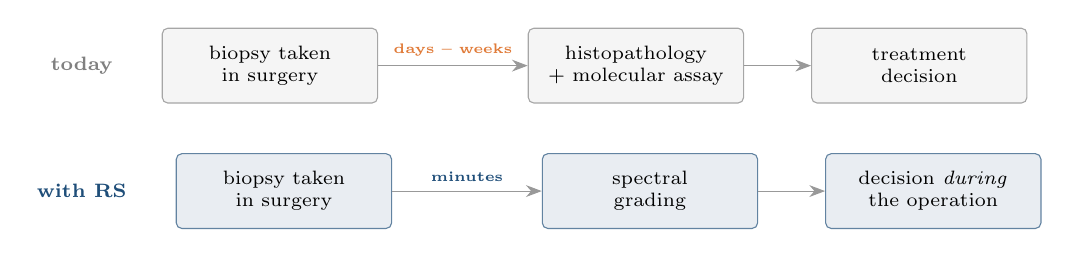
\begin{tikzpicture}[
      node distance=0.45cm and 0.85cm,
      stage/.style={rectangle, rounded corners=2pt, draw=gray!70, fill=gray!8,
                    text width=2.5cm, align=center, font=\scriptsize,
                    minimum height=0.95cm},
      fast/.style={rectangle, rounded corners=2pt, draw=accent!70, fill=accent!10,
                    text width=2.5cm, align=center, font=\scriptsize,
                    minimum height=0.95cm},
      ar/.style={-{Stealth[length=2mm]}, draw=gray!80}]

    \node[font=\scriptsize\bfseries, text=gray] (l1) {today};
    \node[stage, right=0.5cm of l1] (a1) {biopsy taken\\ in surgery};
    \node[stage, right=1.9cm of a1] (b1) {histopathology\\ + molecular assay};
    \node[stage, right=of b1] (c1) {treatment\\ decision};
    \draw[ar] (a1) -- node[above, font=\tiny, text=warm]{\textbf{days -- weeks}} (b1);
    \draw[ar] (b1) -- (c1);

    \node[font=\scriptsize\bfseries, text=accent, below=1.15cm of l1] (l2) {with RS};
    \node[fast, right=0.5cm of l2] (a2) {biopsy taken\\ in surgery};
    \node[fast, right=1.9cm of a2] (b2) {spectral\\ grading};
    \node[fast, right=of b2] (c2) {decision \emph{during}\\ the operation};
    \draw[ar] (a2) -- node[above, font=\tiny, text=accent]{\textbf{minutes}} (b2);
    \draw[ar] (b2) -- (c2);
  \end{tikzpicture}}

  \vspace{0.6em}
  {\small A faster grade means earlier, better-targeted treatment ---
  and plausibly \alert{better outcomes}.}
\end{frame}

% ------------------------------------------------------------ SLIDE 1b ----
% [OPTIONAL] Scoping slide. Drop this if running long -- the same point can be
% made in one spoken sentence over the previous slide.
\begin{frame}{Two different tasks --- this work addresses the harder one}
  \vspace{1.0em}
  \begin{columns}[T]
    \begin{column}{0.48\textwidth}
      \begin{block}{Tumour identification}
        \small
        \emph{Is this tissue tumour or healthy brain?}
        \vspace{0.4em}
        \begin{itemize}\setlength\itemsep{0.25em}\small
          \item already demonstrated intraoperatively
          \item reported accuracies of \textbf{83--99\%}
          \item a large biochemical contrast
        \end{itemize}
      \end{block}
    \end{column}
    \begin{column}{0.48\textwidth}
      \begin{block}{Tumour grading \quad\textnormal{\small(this work)}}
        \small
        \emph{Which molecular subtype is it?}
        \vspace{0.4em}
        \begin{itemize}\setlength\itemsep{0.25em}\small
          \item decides treatment, not just resection
          \item a far more subtle spectral difference
          \item small cohorts make it harder still
        \end{itemize}
      \end{block}
    \end{column}
  \end{columns}
  \vspace{1.0em}
  \centering
  {\small The intraoperative promise rests on the easy task. \alert{Grading is
  where the difficulty --- and the value --- lies.}}
\end{frame}

% ============================================================ SLIDE 2 ======
\begin{frame}{What this work does}
  \vspace{0.6em}
  \begin{columns}[T]
    \begin{column}{0.5\textwidth}
      \textbf{\color{accent}The obstacle}
      \begin{itemize}\setlength\itemsep{0.5em}
        \item 58 biopsy slides, 45 patients
        \item each spectrum is 1738-dimensional
        \item high dimension, small $n$, imbalanced classes
      \end{itemize}
      \vspace{1.2em}
      \textbf{\color{accent}The proposal}
      \begin{itemize}\setlength\itemsep{0.5em}
        \item learn the data distribution with a \textbf{conditional VAE}
        \item generate synthetic spectra to augment training
        \item ask whether this actually helps
      \end{itemize}
    \end{column}
    \begin{column}{0.46\textwidth}
      \textbf{\color{accent}Outline}
      \begin{enumerate}\setlength\itemsep{0.55em}
        \item The data: a hyperspectral cube
        \item Extracting usable tumour spectra
        \item The generative model
        \item Evaluation design
        \item Results and what they mean
      \end{enumerate}
    \end{column}
  \end{columns}
\end{frame}

% ============================================================ SLIDE 3 ======
\begin{frame}{The data is a hyperspectral cube}{Two spatial axes, one spectral axis}
  \centering
  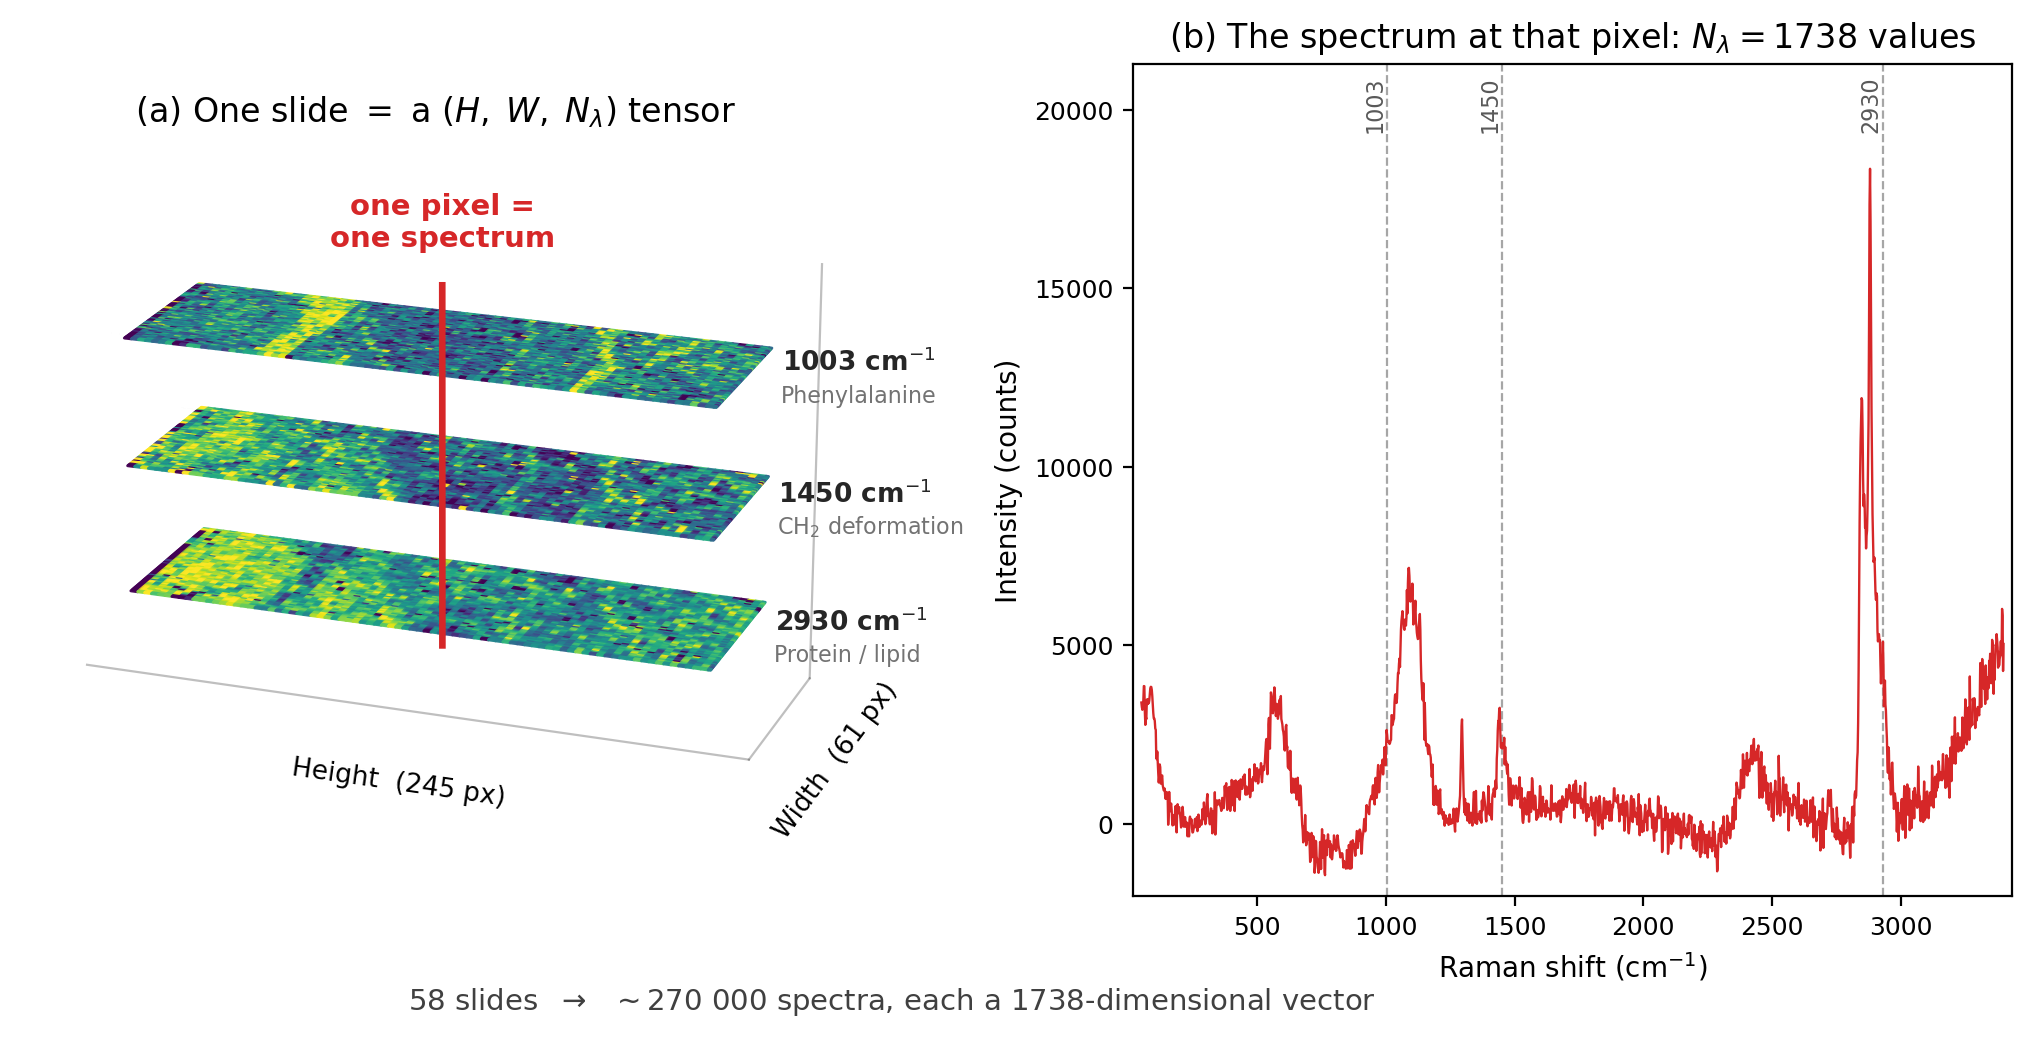
\includegraphics[width=0.98\textwidth]{data_cube.png}
\end{frame}

% ============================================================ SLIDE 4 ======
\begin{frame}{The labels, and the imbalance}
  \vspace{0.3em}
  \begin{columns}[T]
    \begin{column}{0.52\textwidth}
      \small
      \begin{itemize}\setlength\itemsep{0.6em}
        \item Labels come from \textbf{DNA methylation} clustering:
              LGm1--LGm6.
        \item These group into the clinically decisive split:\\
              \textbf{IDH-mutant} (LGm1--3) vs.\ \textbf{IDH-wildtype} (LGm4--6).
        \item Two tasks: \alert{binary IDH status} and the harder
              \alert{6-class subtype}.
      \end{itemize}
      \vspace{0.8em}
      \begin{block}{\small A caveat worth stating}
        \small The labels are \emph{epigenetic}. Nothing guarantees they are
        separable by a Raman spectrum at all.
      \end{block}
    \end{column}
    \begin{column}{0.46\textwidth}
      \centering
      \small
      \begin{tabular}{llcc}
        \toprule
        & \textbf{IDH} & \textbf{Slides} & \textbf{Patients}\\
        \midrule
        LGm1 & mutant   & 5  & 5\\
        LGm2 & mutant   & 11 & 11\\
        LGm3 & mutant   & 9  & 4\\
        \midrule
        LGm4 & wildtype & 13 & 10\\
        LGm5 & wildtype & 15 & 11\\
        LGm6 & wildtype & 5  & 4\\
        \midrule
        \textbf{Total} & & \textbf{58} & \textbf{45}\\
        \bottomrule
      \end{tabular}\\[0.7em]
      \srcnote{LGm1 and LGm6 have 4--5 patients each --- this is what forces
        the cross-validation design later.}
    \end{column}
  \end{columns}
\end{frame}

% ============================================================ SLIDE 5 ======
\begin{frame}{From raw cube to usable spectra}{The processing pipeline}
  \vspace{1.2em}
  \centering
  \resizebox{\textwidth}{!}{%
  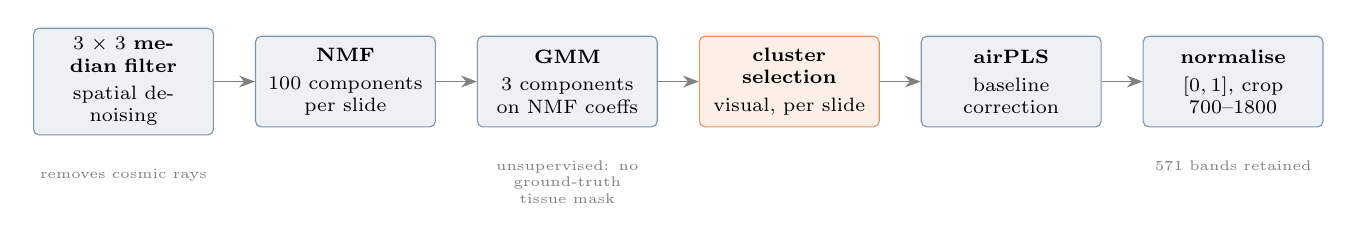
\begin{tikzpicture}[
      node distance=0.62cm and 0.52cm,
      box/.style={rectangle, rounded corners=2pt, draw=accent!60, fill=accent!8,
                  text width=2.05cm, align=center, font=\scriptsize, minimum height=1.15cm},
      sel/.style={rectangle, rounded corners=2pt, draw=warm!80, fill=warm!12,
                  text width=2.05cm, align=center, font=\scriptsize, minimum height=1.15cm},
      ar/.style={-{Stealth[length=2mm]}, draw=gray}]
    \node[box] (a) {$3\times3$ \textbf{median filter}\\[2pt] spatial denoising};
    \node[box, right=of a] (b) {\textbf{NMF}\\[2pt] 100 components\\ per slide};
    \node[box, right=of b] (c) {\textbf{GMM}\\[2pt] 3 components\\ on NMF coeffs};
    \node[sel, right=of c] (d) {\textbf{cluster selection}\\[2pt] visual, per slide};
    \node[box, right=of d] (e) {\textbf{airPLS}\\[2pt] baseline\\ correction};
    \node[box, right=of e] (f) {\textbf{normalise}\\[2pt] $[0,1]$, crop\\ $700$--$1800$};
    \draw[ar] (a)--(b); \draw[ar] (b)--(c); \draw[ar] (c)--(d);
    \draw[ar] (d)--(e); \draw[ar] (e)--(f);
    \node[below=0.30cm of a, font=\tiny, text=gray, text width=2.2cm, align=center]
      {removes cosmic rays};
    \node[below=0.30cm of c, font=\tiny, text=gray, text width=2.4cm, align=center]
      {unsupervised: no ground-truth tissue mask};
    \node[below=0.30cm of f, font=\tiny, text=gray, text width=2.4cm, align=center]
      {571 bands retained};
  \end{tikzpicture}}
  \vspace{1.6em}

  \begin{columns}[c]
    \begin{column}{0.85\textwidth}
      \centering
      \small $\sim$270\,000 raw spectra $\;\longrightarrow\;$
      \alert{$\sim$200\,000} spectra retained as tumour tissue
    \end{column}
  \end{columns}
\end{frame}

% ============================================================ SLIDE 6 ======
\begin{frame}{Step 1 --- spatial median filter}
  \centering
  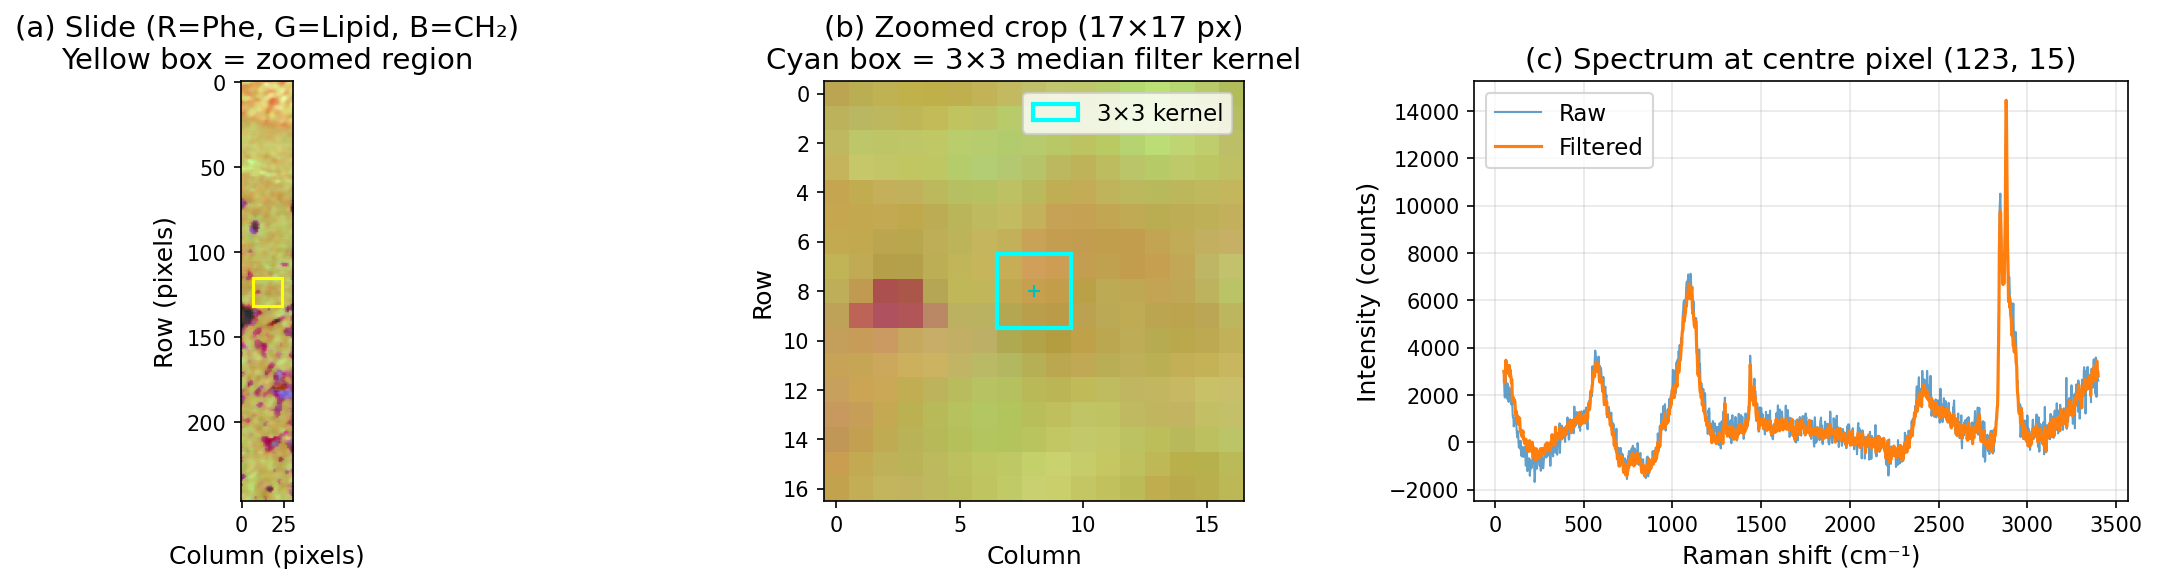
\includegraphics[width=0.97\textwidth]{preprocessing_median_filter_illustration.png}
  \vspace{0.5em}

  \small A $3\times3$ kernel over the \emph{spatial} axes, applied band by band.
  Neighbouring pixels see nearly the same tissue, so the median removes
  cosmic-ray spikes and shot noise \alert{without smoothing the spectral axis}.
\end{frame}

% ============================================================ SLIDE 7 ======
\begin{frame}{Step 2 --- Non-negative Matrix Factorization}{Why non-negativity is the right constraint here}
  \vspace{0.2em}
  \begin{columns}[T]
    \begin{column}{0.46\textwidth}
      Given $M \in \mathbb{R}_+^{m\times n}$ and a rank $r$, find
      \[
        \min_{W \ge 0,\; H \ge 0} \; \lVert M - WH \rVert_F^2
      \]
      \vspace{-0.6em}
      \begin{itemize}\setlength\itemsep{0.45em}
        \small
        \item $W$: $r$ \textbf{endmember} spectra
        \item $H$: how much of each is present at each pixel
      \end{itemize}
    \end{column}
    \begin{column}{0.52\textwidth}
      \begin{block}{\small Why it maps onto the physics}
        \small
        Raman scattering is \alert{additive}: a mixture of molecules produces
        the sum of their spectra, and every contribution is
        \alert{non-negative}. Intensity cannot be negative and a molecule
        cannot be present a negative amount.
      \end{block}
      \vspace{0.3em}
      \small
      Non-negativity also forces \textbf{sparsity} through the KKT conditions,
      giving parts-based components rather than cancelling ones.
      \vspace{0.4em}

      \srcnote{Caveat: we cannot guarantee the components correspond to
        individual chemical species. Here NMF is used only to compress
        each slide before clustering.}
    \end{column}
  \end{columns}
\end{frame}

% ============================================================ SLIDE 8 ======
\begin{frame}{Step 3 --- Gaussian Mixture Model}{Soft clustering in the NMF coefficient space}
  \vspace{0.2em}
  \begin{columns}[T]
    \begin{column}{0.50\textwidth}
      A weighted sum of Gaussians,
      \[
        p(\mathbf{x}) \;=\; \sum_{k=1}^{K} \pi_k\,
          \mathcal{N}(\mathbf{x}\,|\,\mu_k, \Sigma_k)
      \]
      with responsibilities
      \[
        \gamma(z_k) = \frac{\pi_k\,\mathcal{N}(\mathbf{x}|\mu_k,\Sigma_k)}
                           {\sum_j \pi_j\,\mathcal{N}(\mathbf{x}|\mu_j,\Sigma_j)}
      \]
      \small fitted by \textbf{Expectation-Maximization}, alternating
      between the assignments and the parameters.
    \end{column}
    \begin{column}{0.48\textwidth}
      \begin{block}{\small The input is not the spectrum}
        \small
        The GMM is fitted to the \alert{NMF coefficients} $H$, not the 1738
        raw bands: $100$ dimensions instead of $1738$, which makes the
        covariance estimates tractable.
      \end{block}
      \vspace{0.5em}
      \small
      $K=3$ components per slide, fitted \textbf{independently for each
      slide} --- so instrument drift between acquisitions cannot leak
      between slides.
    \end{column}
  \end{columns}
\end{frame}

% ============================================================ SLIDE 9 ======
\begin{frame}{Step 4 --- selecting the tumour clusters}
  \vspace{0.4em}
  \centering
  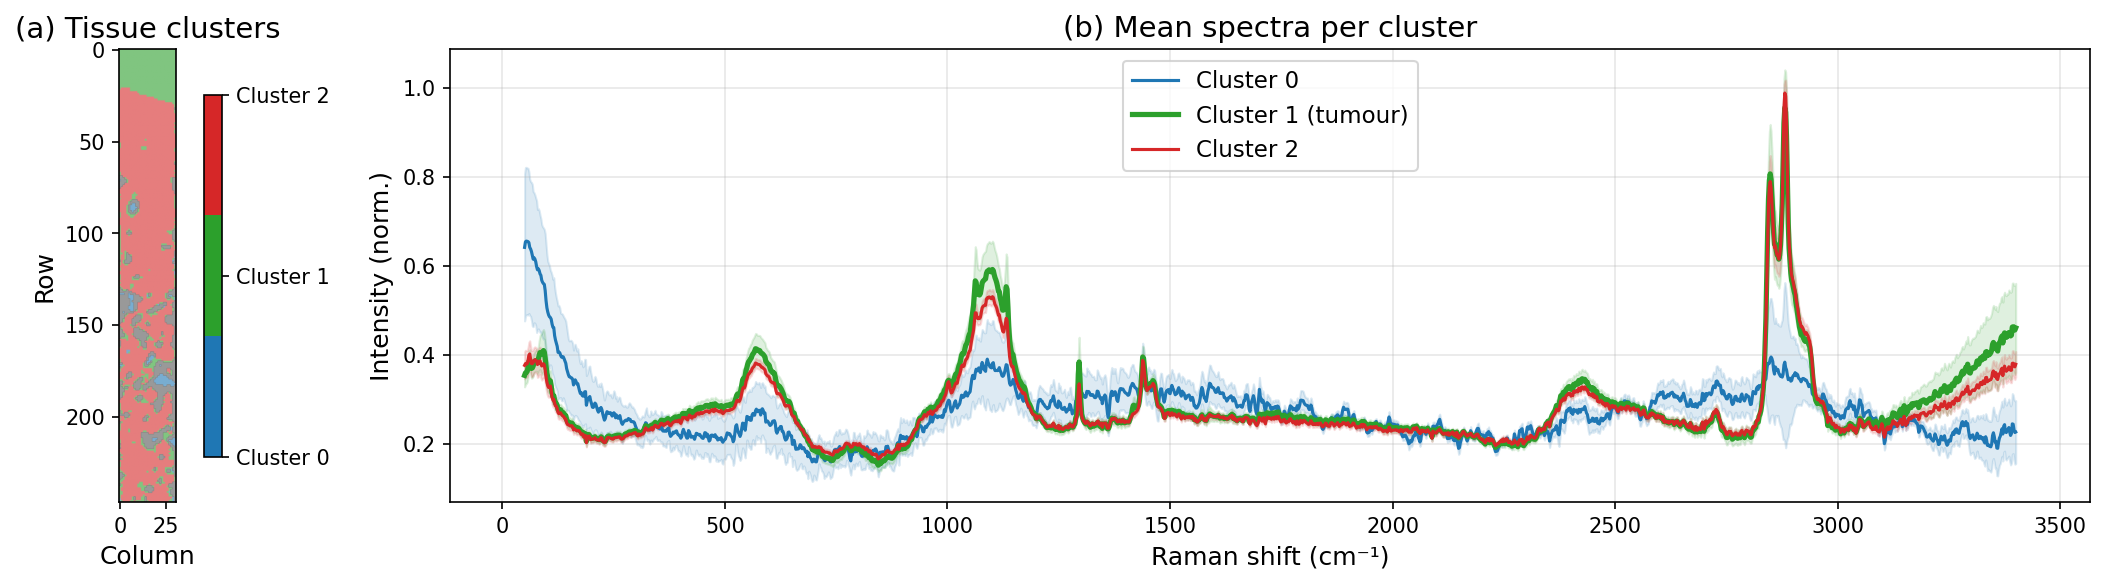
\includegraphics[width=0.93\textwidth]{preprocessing_cluster_spectra.png}
  \vspace{0.8em}

  \small Each cluster is inspected \alert{spatially} --- is it contiguous
  tissue or scattered noise? --- and \alert{spectrally} --- is the signal
  strong? Here the blue cluster is weak background and is discarded.
\end{frame}

% ============================================================ SLIDE 10 =====
\begin{frame}{The generative model: a conditional VAE}{From function approximation to distribution estimation}
  \vspace{0.3em}
  \begin{columns}[T]
    \begin{column}{0.50\textwidth}
      \small
      An autoencoder compresses and reconstructs. A \textbf{variational}
      autoencoder additionally constrains the latent space to follow
      $\mathcal{N}(0,I)$:
      \[
        \mathcal{L}_{\text{ELBO}} =
        \underbrace{\mathbb{E}_{q}[\log p_\theta(x|z)]}_{\text{reconstruction}}
        \;-\;
        \underbrace{D_{KL}(q_\phi(z|x)\,\|\,p(z))}_{\text{regularisation}}
      \]
      \vspace{-0.3em}
      \begin{itemize}\setlength\itemsep{0.4em}
        \item sampling is not differentiable, so we use the
              \textbf{reparameterisation trick}
              $z = \mu + \sigma \odot \epsilon$
        \item \textbf{conditional}: the label $y$ is fed to the decoder, so we
              can ask for a spectrum \emph{of a given class}
      \end{itemize}
    \end{column}
    \begin{column}{0.48\textwidth}
      \begin{block}{\small Why the KL term is what makes it a generator}
        \small
        To generate, we sample $z\sim\mathcal{N}(0,I)$ and decode. That is only
        meaningful if the decoder was \alert{trained on codes distributed that
        way}. A plain autoencoder leaves gaps in the latent space that decode
        to noise; the KL term pulls the encoded distribution onto the prior.
      \end{block}
      \vspace{0.4em}
      \small The weight $\beta$ controls that pull --- and, as we will see,
      buys regularity at the cost of \alert{variance}.
    \end{column}
  \end{columns}
\end{frame}

% ============================================================ SLIDE 11 =====
\begin{frame}{Architecture}{1D convolutions along the wavenumber axis}
  \vspace{0.2em}
  \centering
  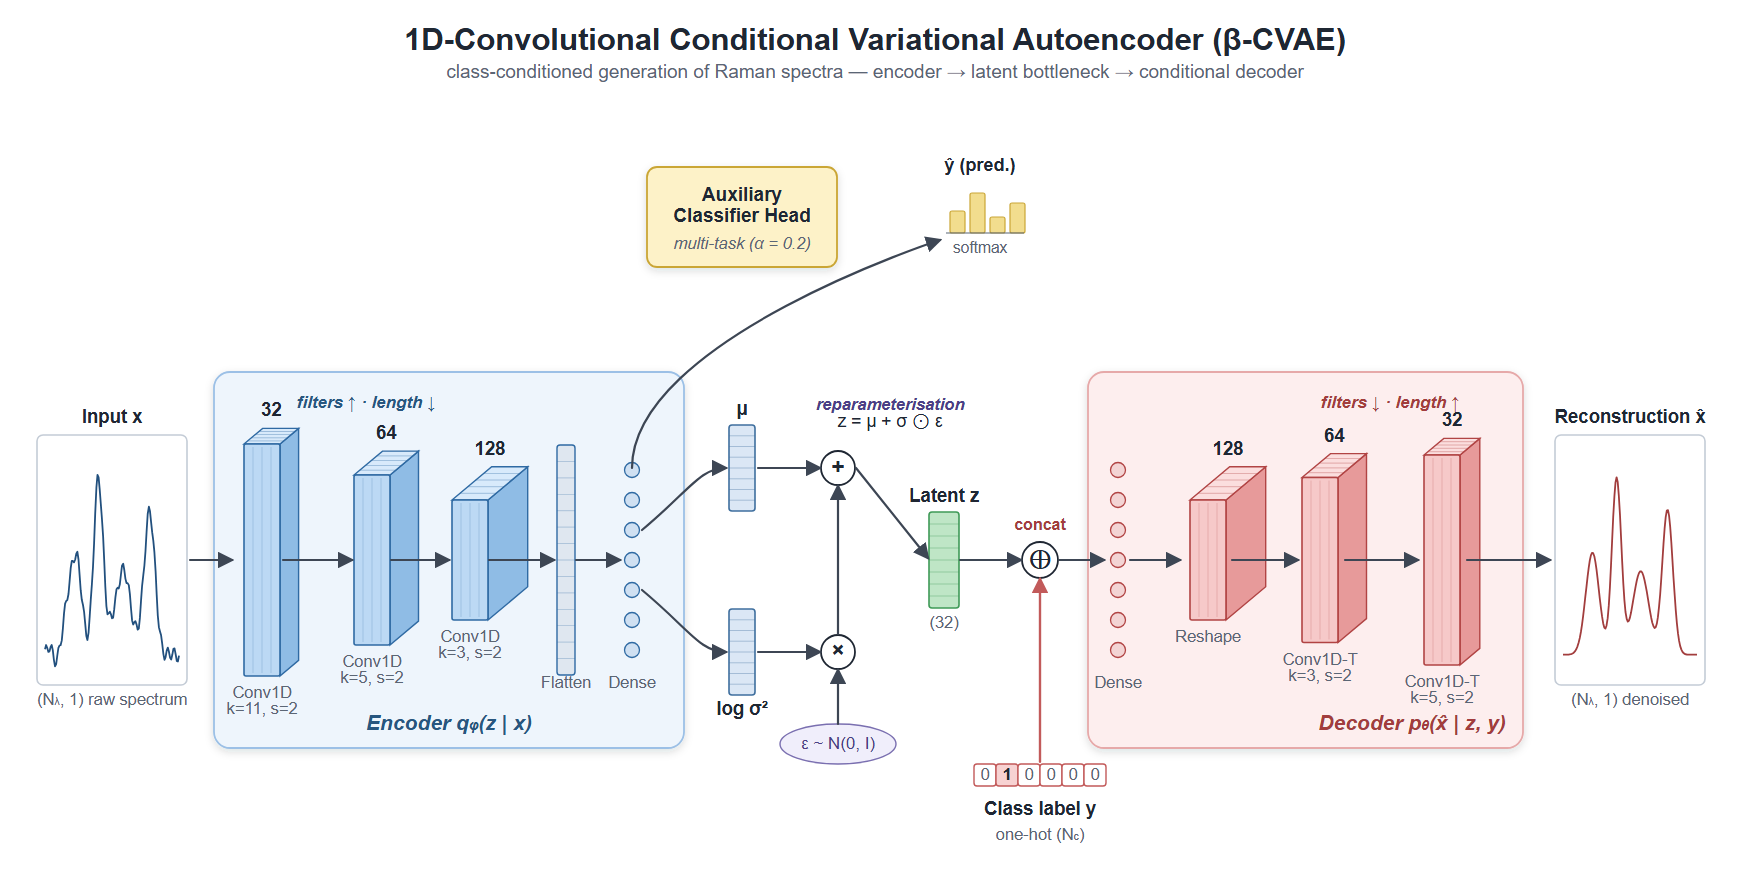
\includegraphics[width=0.86\textwidth]{cvae_architecture.png}
  \vspace{0.6em}

  \small
  A Raman band is a \alert{local} feature whose position drifts between
  acquisitions --- weight sharing gives translation equivariance.
\end{frame}

% ============================================================ SLIDE 12 =====
\begin{frame}{Training objective}{Three terms, one network}
  \vspace{0.8em}
  \[
    \mathcal{L}_{\text{total}}
      = \underbrace{\mathcal{L}_{\text{recon}}}_{\text{fidelity}}
      \;+\; \beta \cdot \underbrace{D_{KL}\!\left(q_\phi(z|x)\,\|\,p(z)\right)}_{\text{usable latent space}}
      \;+\; \alpha \cdot \underbrace{\mathcal{L}_{\text{class}}}_{\text{class-aware encoder}}
  \]
  \vspace{0.6em}
  \begin{columns}[T]
    \begin{column}{0.32\textwidth}
      \textbf{\small Reconstruction}\\[0.3em]
      {\small $\gamma\,\text{MSE} + (1-\gamma)\,\text{CosineLoss}$\\[0.4em]
      MSE matches amplitude, cosine matches \emph{shape}.}
    \end{column}
    \begin{column}{0.32\textwidth}
      \textbf{\small KL divergence}\\[0.3em]
      {\small $\beta = 2$: deliberately $>1$, so the latent space is regular
      enough to sample from.}
    \end{column}
    \begin{column}{0.32\textwidth}
      \textbf{\small Auxiliary classifier}\\[0.3em]
      {\small $\alpha = 0.2$: encourages class-discriminative features.
      At $0.5$ the encoder overfits the classification task early.}
    \end{column}
  \end{columns}
  \vspace{1.0em}
  \centering
  \srcnote{Adam optimizer, 70 epochs, batch 256, latent dimension $d=32$.
    Dynamic augmentation at train time: within-class mixup and $\pm3$ band
    spectral shift, simulating calibration drift.}
\end{frame}

% ============================================================ SLIDE 13 =====
\begin{frame}{Evaluation --- splitting the data}
  \centering
  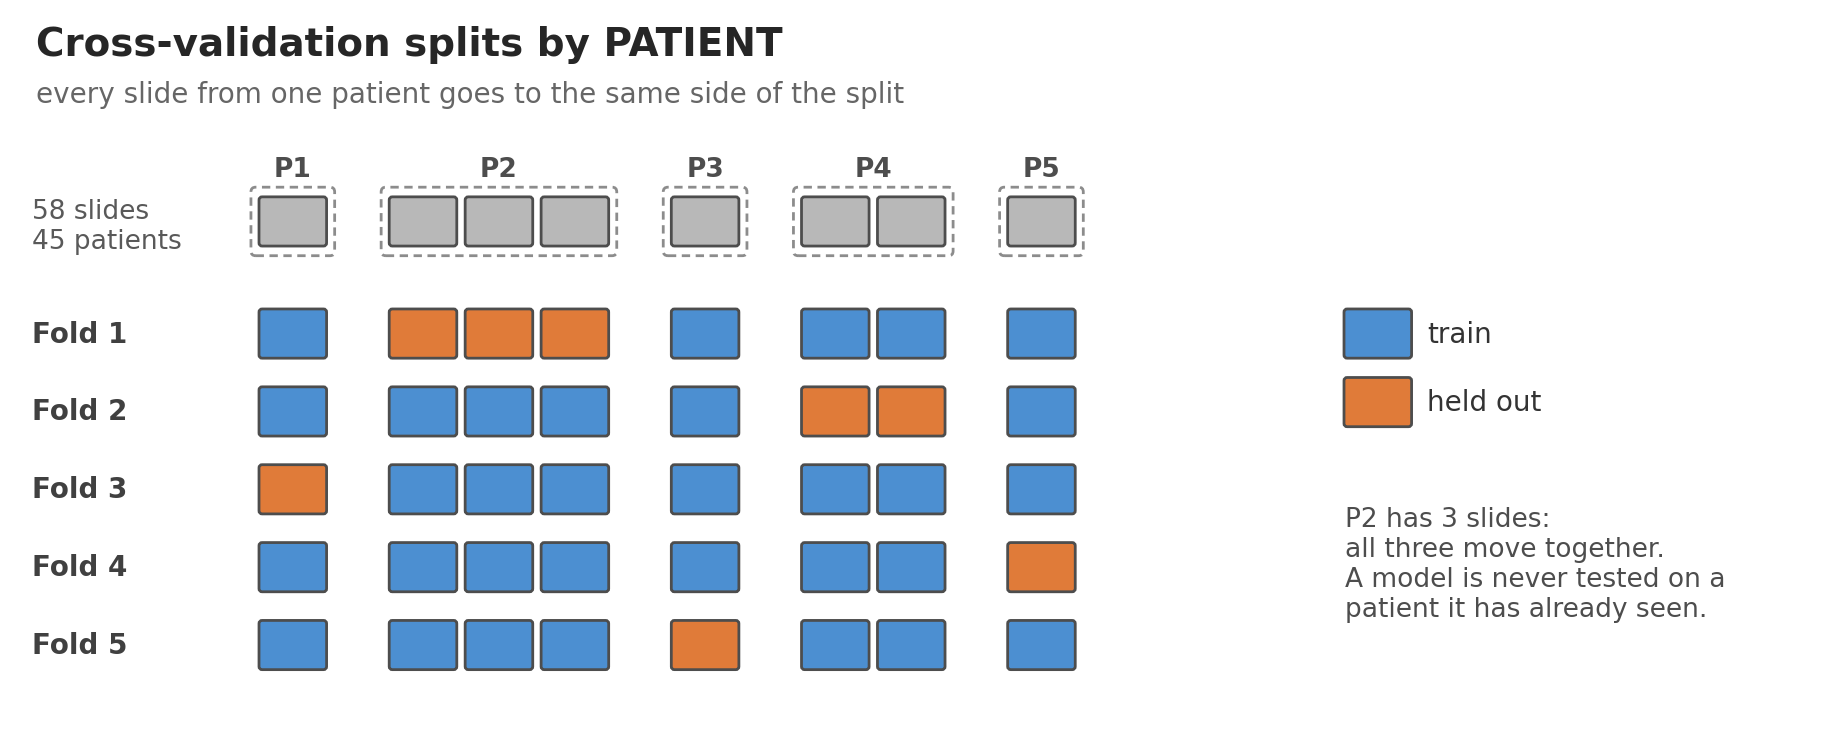
\includegraphics[width=0.94\textwidth]{cv_design.png}
  \vspace{0.4em}

  \small Class-stratified, but \alert{not a partition}: LGm1 and LGm6 have so
  few patients that some appear in two test folds. Patient separation is never
  relaxed.
\end{frame}

% ============================================================ SLIDE 14 =====
\begin{frame}{Evaluation --- estimating uncertainty}
  \centering
  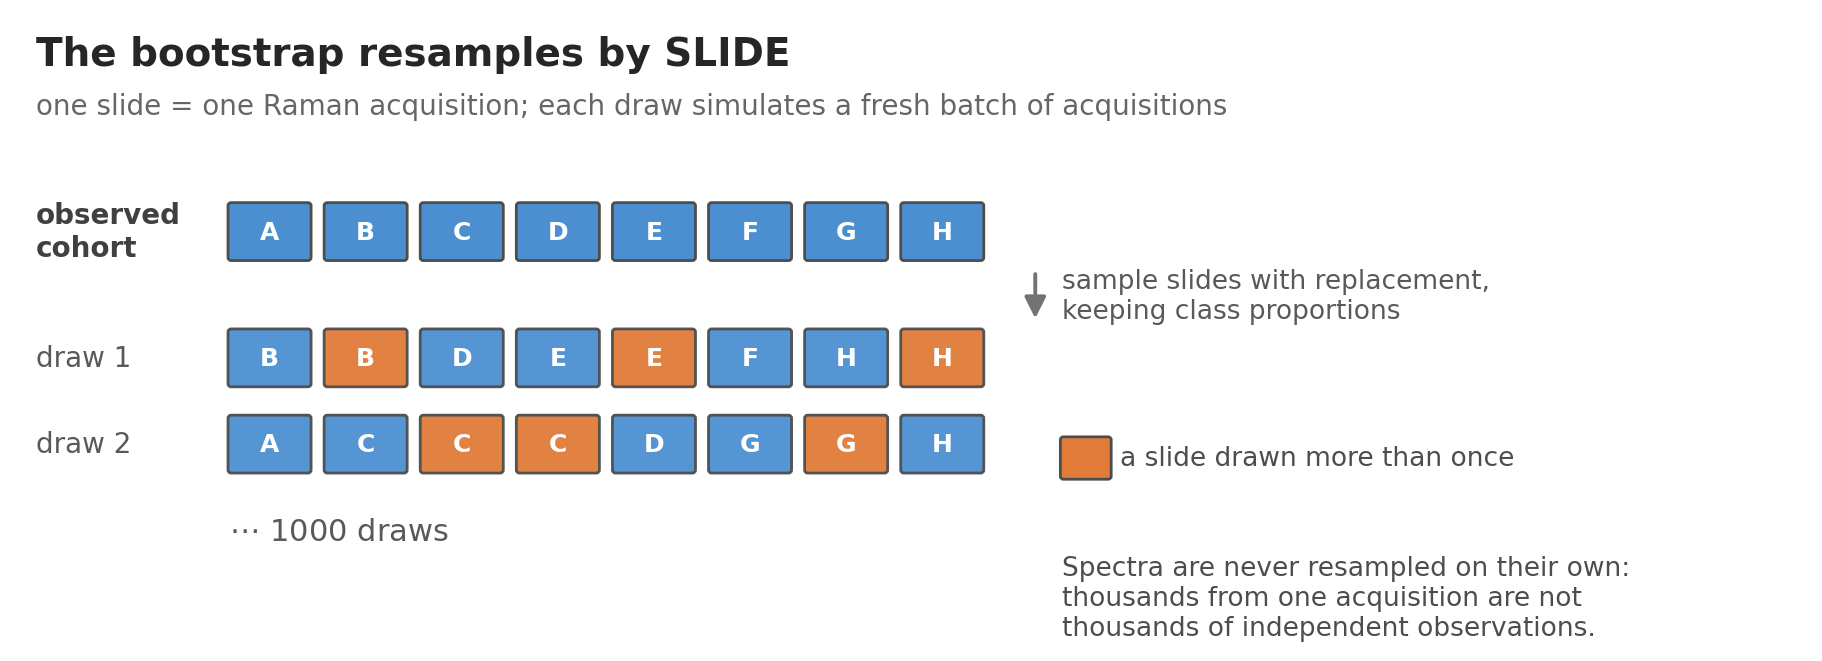
\includegraphics[width=0.94\textwidth]{bootstrap_design.png}
  \vspace{0.3em}

  \small
  \textbf{Two units, deliberately.} Splitting asks \emph{is the test data
  unseen?} $\rightarrow$ the strictest unit, the patient. Resampling asks
  \emph{how much would this number move?} $\rightarrow$ the acquisition, which
  is what drives spectral variability.
\end{frame}

% ============================================================ SLIDE 15 =====
\begin{frame}{Results --- binary IDH classification}
  \vspace{0.1em}
  \centering
  \footnotesize
  \begin{tabular}{llccc}
    \toprule
    \emph{Model} & \emph{Regimen} & \emph{Bal. Acc.} & \emph{$\Delta$ vs TR/TR} & \emph{95\% CI}\\
    \midrule
    \multirow{3}{*}{RF + SVM} & TR/TR  & $0.688$ & --- & ---\\
                              & TS/TR  & $0.431$ & $-0.257$\alert{*} & $[-0.330, -0.180]$\\
                              & TSR/TR & $0.699$ & $+0.011$ & $[-0.015, +0.037]$\\
    \midrule
    \multirow{3}{*}{Random Forest} & TR/TR  & $0.734$ & --- & ---\\
                              & TS/TR  & $0.669$ & $-0.065$ & $[-0.148, +0.017]$\\
                              & TSR/TR & $\mathbf{0.742}$ & $+0.008$ & $[-0.001, +0.019]$\\
    \midrule
    \multirow{3}{*}{XGBoost}  & TR/TR  & $0.742$ & --- & ---\\
                              & TS/TR  & $0.622$ & $-0.120$\alert{*} & $[-0.191, -0.051]$\\
                              & TSR/TR & $\mathbf{0.746}$ & $+0.004$ & $[-0.004, +0.013]$\\
    \midrule
    \multirow{3}{*}{1D-CNN}   & TR/TR  & $0.588$ & --- & ---\\
                              & TS/TR  & $0.398$ & $-0.190$\alert{*} & $[-0.299, -0.077]$\\
                              & TSR/TR & $0.602$ & $+0.014$ & $[-0.055, +0.086]$\\
    \midrule
    CbR & --- & $0.619$ & --- & $[+0.548, +0.681]$\\
    \bottomrule
  \end{tabular}\\[0.5em]
  \srcnote{TR/TR real only $\cdot$ TS/TR synthetic only $\cdot$ TSR/TR both.
    \alert{*} marks a 95\% CI excluding zero. Slide-level balanced accuracy.}
\end{frame}

% ============================================================ SLIDE 16 =====
\begin{frame}{What the synthetic spectra actually look like}
  \vspace{0.2em}
  \begin{columns}[c]
    \begin{column}{0.5\textwidth}
      \centering
      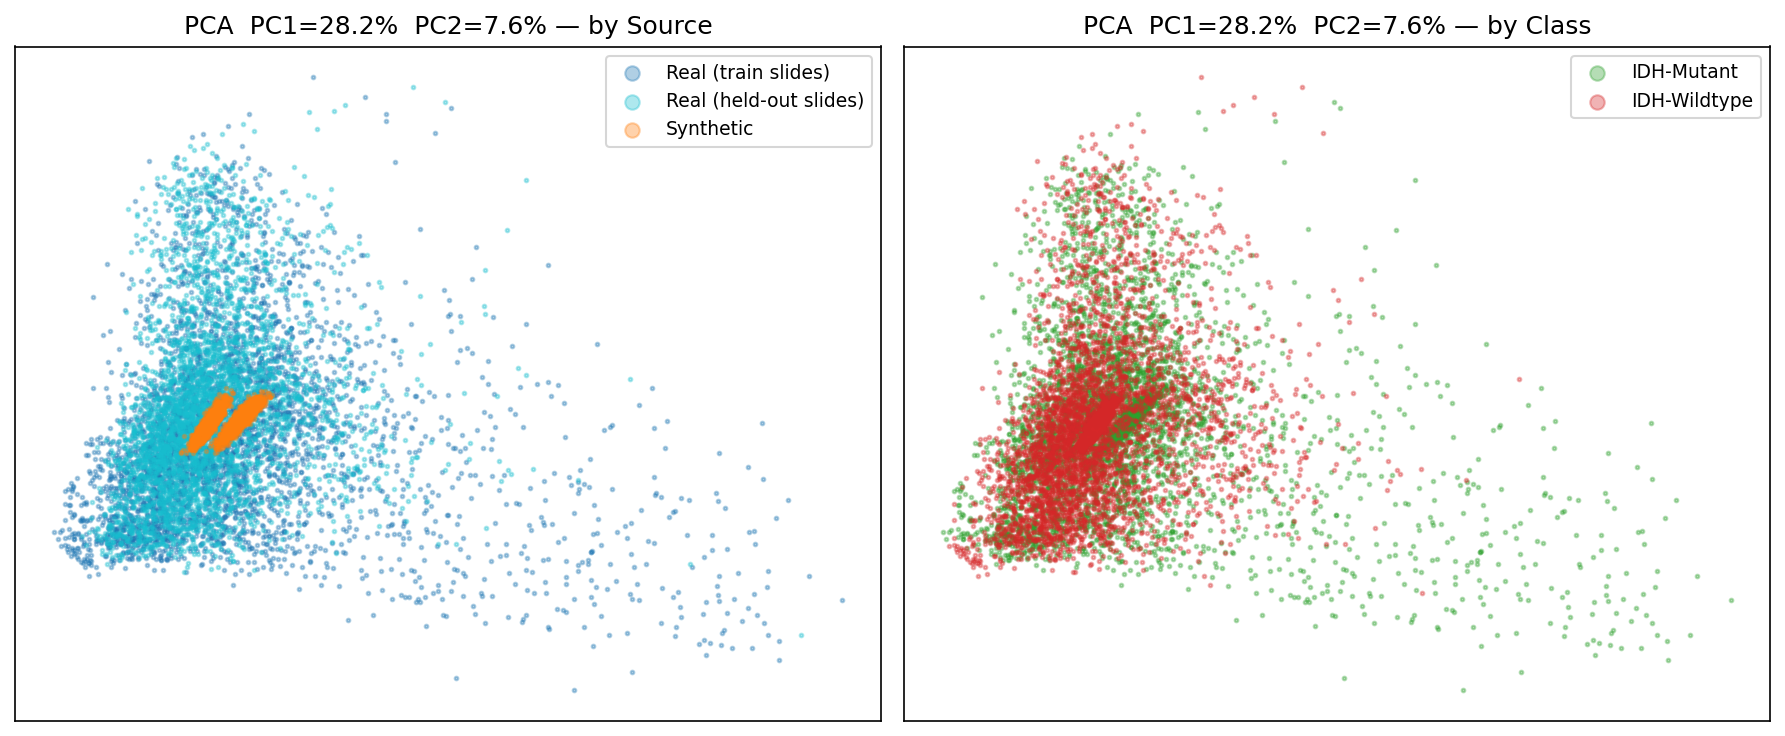
\includegraphics[width=\linewidth]{exp201_fold0_pca.png}\\[0.3em]
      \srcnote{PCA --- distances are meaningful}
    \end{column}
    \begin{column}{0.5\textwidth}
      \centering
      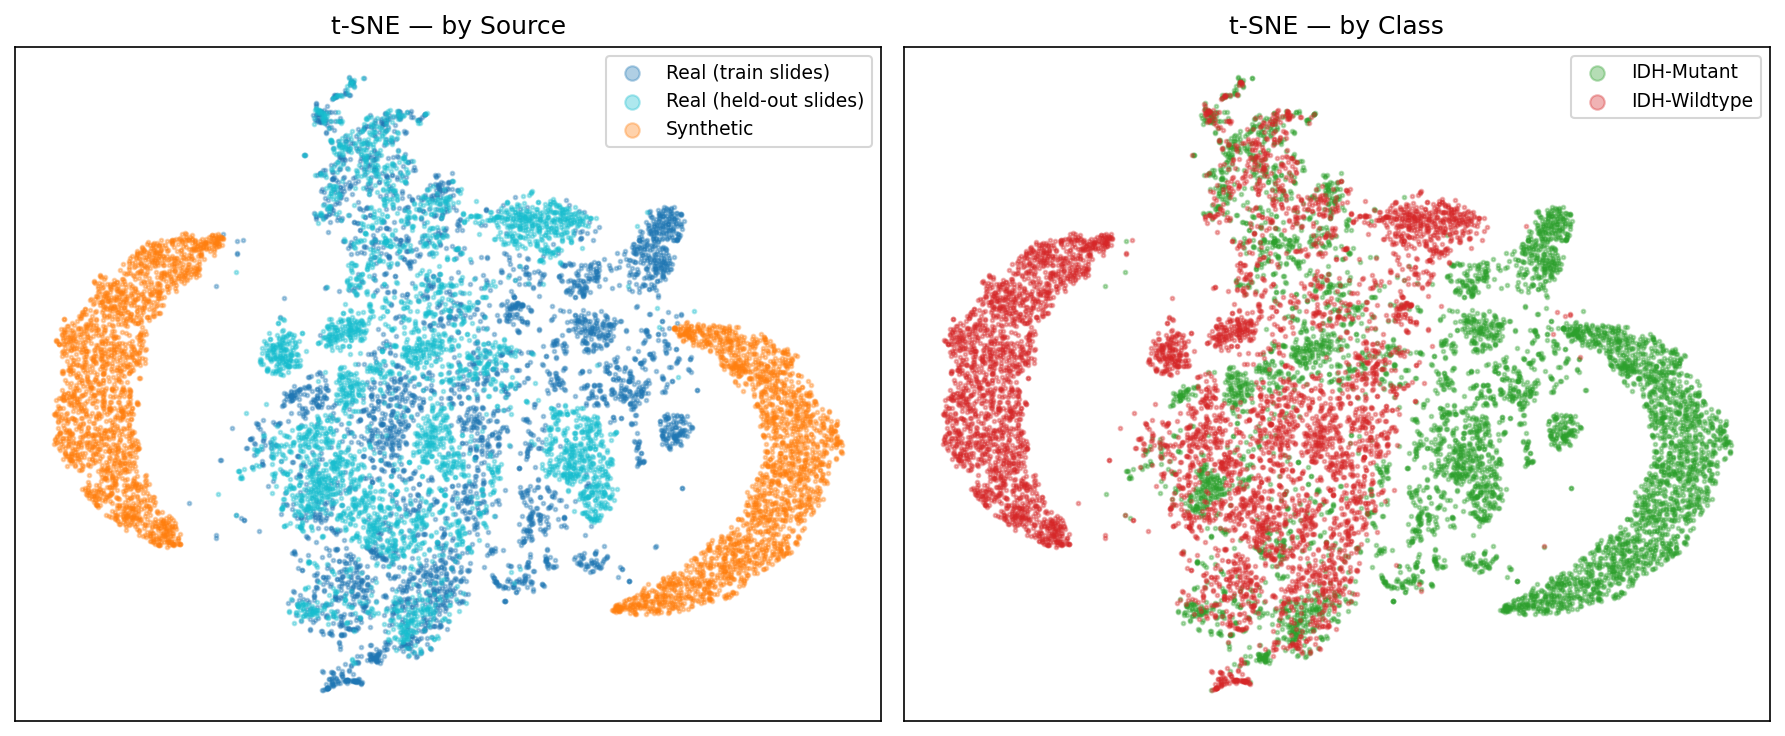
\includegraphics[width=\linewidth]{exp201_fold0_tsne.png}\\[0.3em]
      \srcnote{$t$-SNE --- only \emph{local} neighbourhoods are meaningful}
    \end{column}
  \end{columns}
  \vspace{0.5em}
  \small
  \begin{itemize}\setlength\itemsep{0.25em}
    \item Real train and held-out spectra are \alert{intermixed} --- the gap is
          not an artefact of the split.
    \item In PCA the synthetic spectra collapse to a narrow sliver
          \alert{inside} the real cloud: mode collapse, not drift.
    \item $t$-SNE separates them into two arcs --- but inter-cluster distance
          there is \alert{not} interpretable.
  \end{itemize}
\end{frame}

% ============================================================ SLIDE 17 =====
\begin{frame}{Conclusions}
  \vspace{0.4em}
  \begin{columns}[T]
    \begin{column}{0.48\textwidth}
      \textbf{\color{accent}What the evidence supports}
      \begin{itemize}\setlength\itemsep{0.4em}\small
        \item Augmentation moves accuracy \alert{up in sign} for every model and
              both tasks.
        \item The generator captures class-mean structure: synthetic-only
              training stays well above chance.
        \item CbR shows the latent space retains class information without any
              discriminative classifier.
      \end{itemize}
    \end{column}
    \begin{column}{0.48\textwidth}
      \textbf{\color{accent}What it does not}
      \begin{itemize}\setlength\itemsep{0.4em}\small
        \item The gains are \alert{not statistically significant} --- essentially
              every 95\% CI includes zero.
        \item Synthetic spectra \alert{cannot replace} real ones: TS/TR is below
              TR/TR everywhere.
        \item Diagnosis: good fidelity, \alert{poor diversity}.
      \end{itemize}
    \end{column}
  \end{columns}
  \vspace{1.0em}
  \begin{block}{\small Where this goes next}
    \small
    The failure is specific and therefore actionable: the $\beta$ weighting buys
    latent regularity at the cost of the variance shown missing. A $\beta$ sweep
    is the obvious next experiment --- $\beta$ was held at $2$ throughout.
    Beyond that: diffusion models, and multi-site data.
  \end{block}
\end{frame}

% ============================================================ CLOSING =====
{
\setbeamertemplate{footline}{}
\begin{frame}[plain]
  \vfill
  \begin{center}
    {\LARGE\bfseries\color{accent} Thank you}\\[1.2em]
    {\large Questions?}\\[2.0em]
    \small\color{gray}
    Preprint: arXiv:2607.10196\\
    Code: \texttt{glioma-synthetic-data}
  \end{center}
  \vfill
\end{frame}
}

% ============================================================ BACKUP ======
\appendix

\begin{frame}{Backup --- airPLS baseline correction}
  \centering
  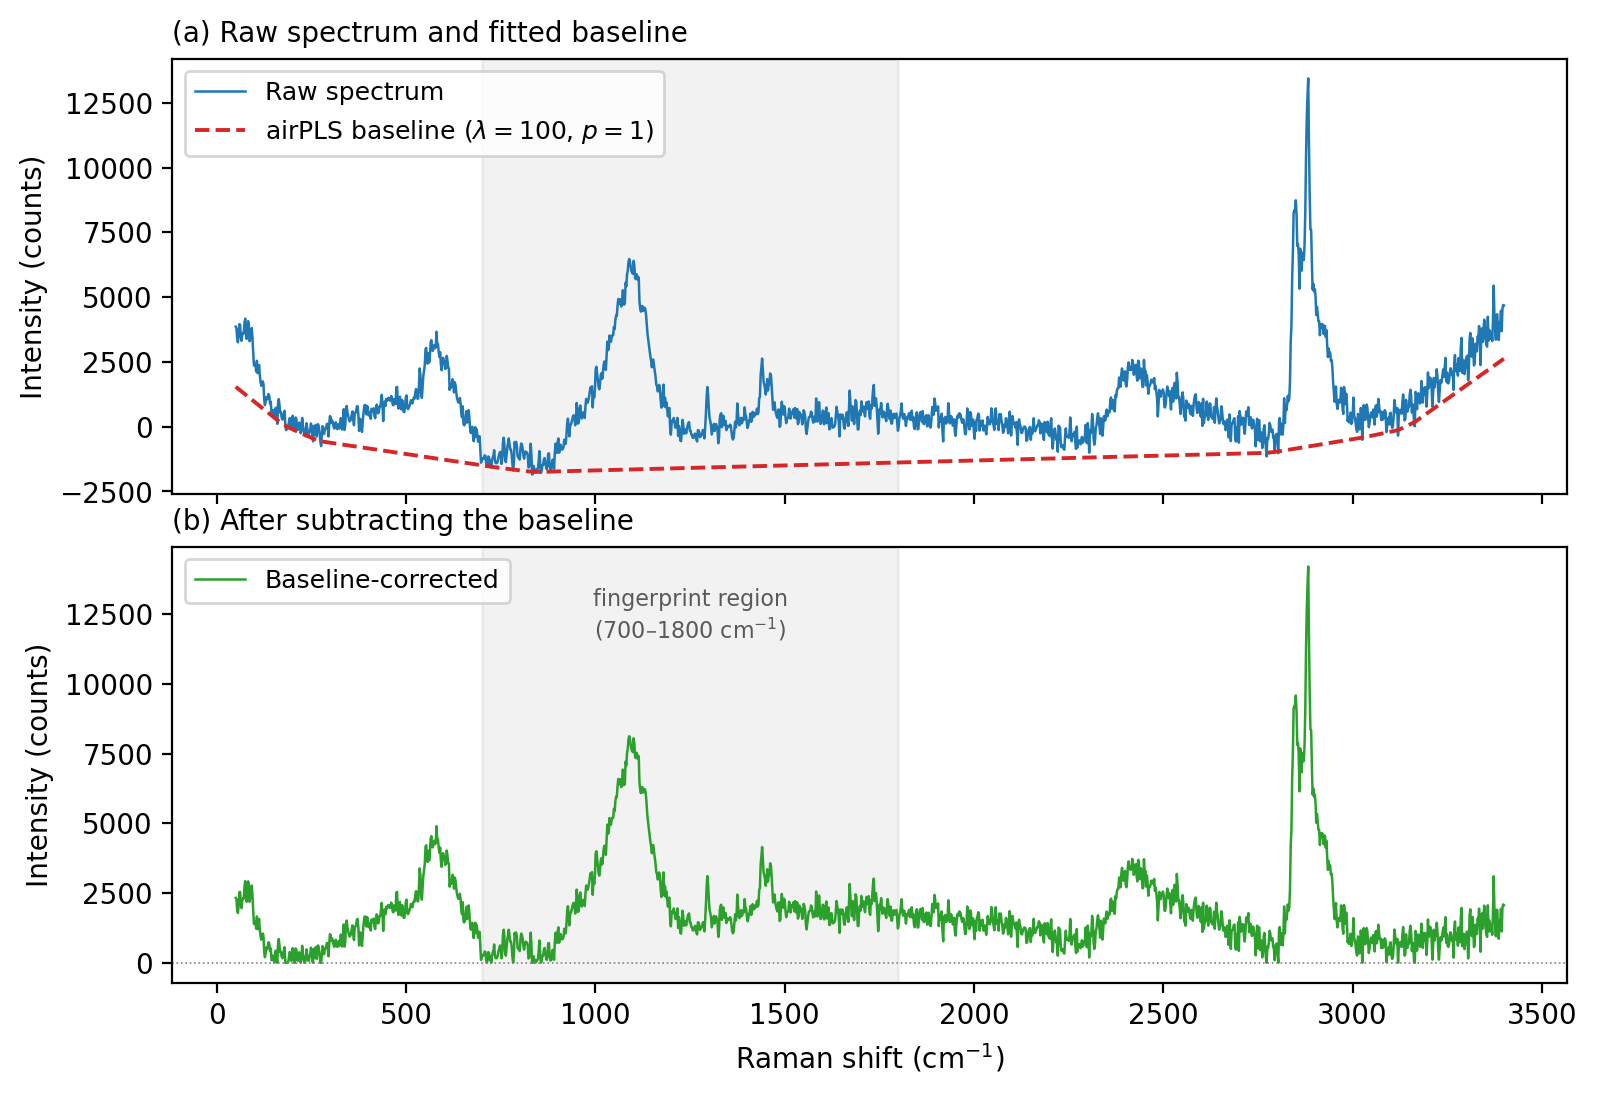
\includegraphics[width=0.70\textwidth]{airpls_baseline_correction.png}\\[0.2em]
  \srcnote{$\lambda=100$, $p=1$. The baseline tracks the lower envelope, so
    subtracting it does not remove peaks.}
\end{frame}

\begin{frame}{Backup --- fidelity is good, diversity is not}
  \centering
  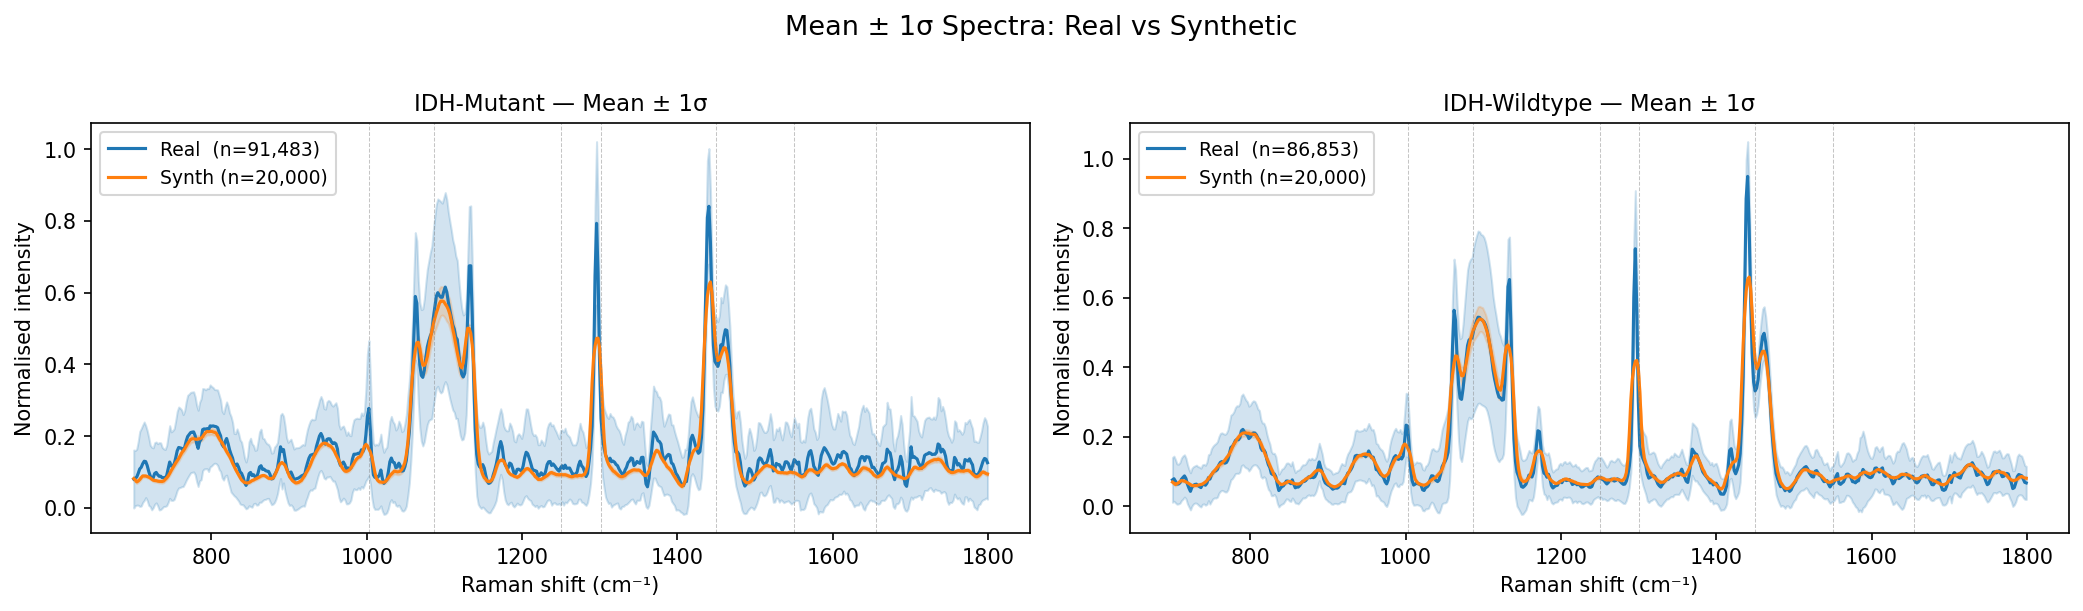
\includegraphics[width=0.95\textwidth]{exp201_fold0_mean_std.png}\\[0.3em]
  \small The mean spectra track closely. The synthetic $\pm1\sigma$ envelope is
  \alert{barely visible} next to the real one --- this is the whole finding, in
  one picture.
\end{frame}

\begin{frame}{Backup --- 6-class sub-grading}
  \vspace{0.3em}
  \centering
  \small
  \begin{tabular}{llccc}
    \toprule
    \emph{Model} & \emph{Regimen} & \emph{Bal. Acc.} & \emph{$\Delta$} & \emph{95\% CI}\\
    \midrule
    \multirow{3}{*}{RF + SVM} & TR/TR & $0.289$ & --- & ---\\
      & TS/TR  & $0.102$ & $-0.186$\alert{*} & $[-0.275, -0.094]$\\
      & TSR/TR & $0.301$ & $+0.012$ & $[-0.012, +0.040]$\\
    \midrule
    \multirow{3}{*}{XGBoost} & TR/TR & $0.268$ & --- & ---\\
      & TS/TR  & $0.251$ & $-0.018$ & $[-0.072, +0.041]$\\
      & TSR/TR & $0.266$ & $-0.002$ & $[-0.009, +0.004]$\\
    \midrule
    \multirow{3}{*}{1D-CNN} & TR/TR & $0.224$ & --- & ---\\
      & TS/TR  & $0.075$ & $-0.149$\alert{*} & $[-0.240, -0.062]$\\
      & TSR/TR & $0.249$ & $+0.025$ & $[-0.100, +0.158]$\\
    \bottomrule
  \end{tabular}\\[0.5em]
  \srcnote{Chance level is $0.167$. Accuracy degrades with granularity ---
    the same pattern the literature reports.}
\end{frame}

\begin{frame}{Backup --- latent dimension makes no difference}
  \vspace{0.3em}
  \centering
  \small
  \begin{tabular}{lcccc}
    \toprule
    \emph{Model} & $d=16$ & $d=32$ & $d=64$ & \emph{regimen}\\
    \midrule
    RF + SVM & $0.695$ & $0.699$ & $0.709$ & TSR/TR\\
    Random Forest & $0.735$ & $0.742$ & $0.734$ & TSR/TR\\
    XGBoost & $0.745$ & $0.746$ & $0.745$ & TSR/TR\\
    1D-CNN & $0.635$ & $0.602$ & $0.700$\alert{*} & TSR/TR\\
    \midrule
    CbR & $0.616$ & $0.619$ & $0.621$ & ---\\
    \bottomrule
  \end{tabular}\\[0.6em]
  \small No trend across $d$. CbR is flat to within $0.005$ despite depending on
  the latent representation directly.\\[0.3em]
  \srcnote{The single starred result is the least stable classifier, against a
    baseline that itself differs in that run; with twelve comparisons and no
    multiplicity correction, one such interval is about what chance predicts.}
\end{frame}

\begin{frame}{Backup --- how does this compare to the literature?}
  \vspace{0.4em}
  \centering
  \small
  \begin{tabular}{llcc}
    \toprule
    \emph{Study} & \emph{Task} & \emph{Validation} & \emph{Acc.}\\
    \midrule
    Uckermann et al. & IDH-mut vs.\ wt & 36 frozen sections & $89\%$\\
    Sciortino et al. & IDH-mut vs.\ wt & --- & $87\%$\\
    Livermore et al. & IDH status & LOPOCV & $91/95$ sens/spec\\
    \midrule
    Riva et al. & tumour vs.\ normal & \alert{LOPOCV}, RF/GB & $83\%$\\
    \textbf{This work} & IDH-mut vs.\ wt & \alert{patient-level 5-fold} & $\mathbf{74\%}$\\
    \bottomrule
  \end{tabular}\\[0.7em]
  \small
  Most published numbers validate over \alert{spectra}, placing spectra from one
  patient on both sides of the split. The honest comparator is Riva et al.:
  patient-level, same model families, the \emph{easier} task.
\end{frame}

\end{document}
